
\newpage
\section{Casos de uso}
El la siguiente sección se define y describen los Actores,funciones y esenarios, describiendo su funcionalidad e interacción dentro de la aplicación.\par
\vspace{5mm}
\begin{figure}[h!]
	\centering
	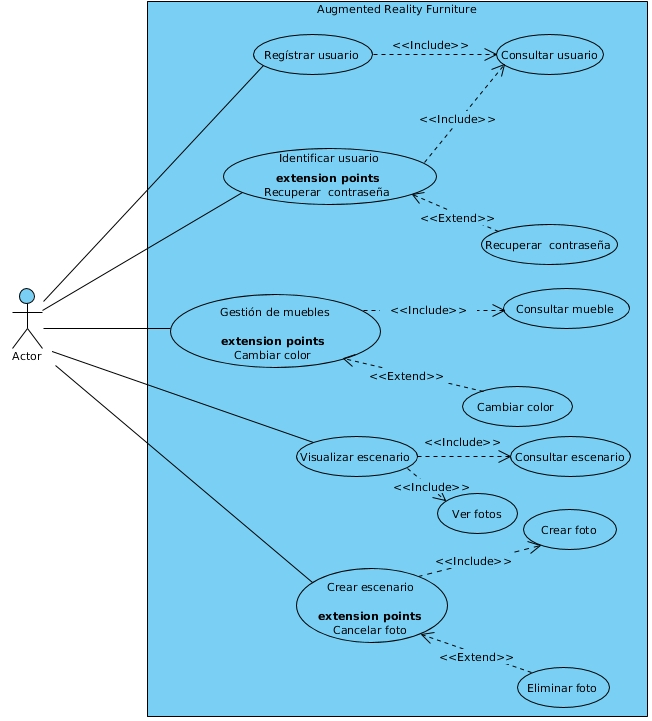
\includegraphics[width=15cm,height=17cm]{imagenes/analisis/casosDeUso.jpg}
	\caption{Casos de uso.}
	\label{fig:analogo}
\end{figure}  
\newpage

\subsection{Caso de uso 1 :} \textit{Login}
\begin{figure}[h!]
	\centering
	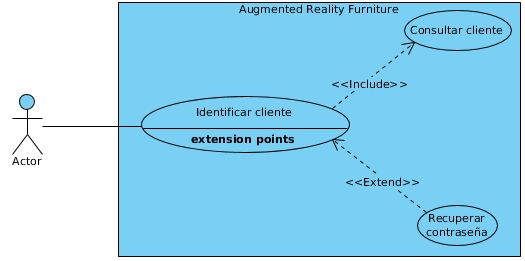
\includegraphics[width=12cm,height=6cm]{imagenes/analisis/login.jpg}
	\caption{CU01 Login.}
	\label{fig:analogo}
\end{figure}  

\subsection{Caso de uso 2 :} \textit{Registrar usuario} 
\vspace{5mm} 	
\begin{figure}[h!]
	\centering
	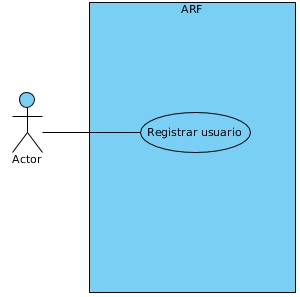
\includegraphics[width=12cm,height=6cm]{imagenes/analisis/registrarUsuario.jpg}
	\caption{CU02 Registrar un usuario.}
	\label{fig:analogo}
\end{figure} 
\newpage
\subsection{Caso de uso 3 :} \textit{Seleccionar mueble} 
\vspace{5mm}
\begin{figure}[h!]
	\centering
	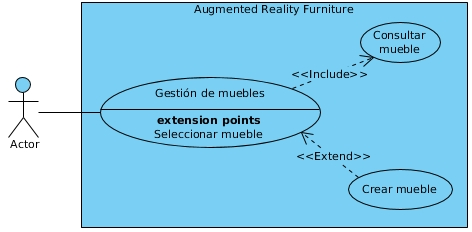
\includegraphics[width=12cm,height=6cm]{imagenes/analisis/seleccionarMueble.jpg}
	\caption{CU3 Seleccionar mueble.}
	\label{fig:analogo}
\end{figure}

\subsection{Caso de uso 4 :}\textit{Visualizar escenario} 
\vspace{5mm}
\begin{figure}[h!]
	\centering
	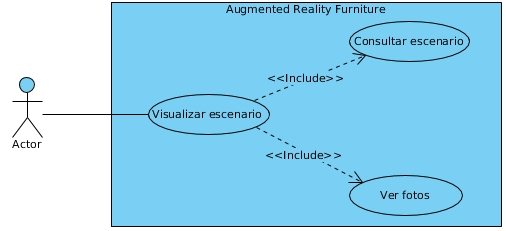
\includegraphics[width=12cm,height=6cm]{imagenes/analisis/visualizarEscenario.jpg}
	\caption{CU04 Gestionar escenario.}
	\label{fig:analogo}
\end{figure}

\subsection{Caso de uso 4 :}\textit{Crear escenario} 
\vspace{5mm}
\begin{figure}[h!]
	\centering
	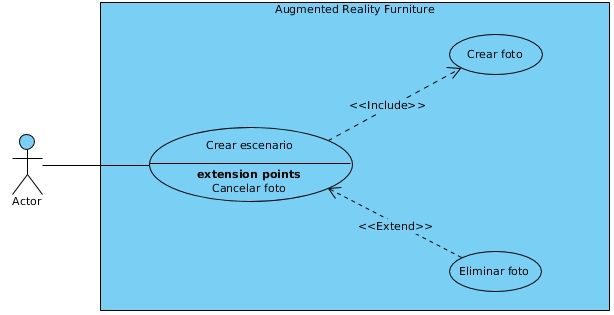
\includegraphics[width=12cm,height=6cm]{imagenes/analisis/crearEscenario.jpg}
	\caption{CU04 Gestionar escenario.}
	\label{fig:analogo}
\end{figure}